\chapter{Verwandte Arbeiten}\label{sec:related}

In diesem Kapitel wird ein Überblick über verwandte Arbeiten gegeben. Dazu wird zunächst die Arbeit von Henseler \cite{bachelor:henseler:gaze-ebikes} vorgestellt, die sich speziell mit der Blickrichtungsbestimmung von Radfahrenden beschäftigt. Anschließend werden Arbeiten vorgestellt, die sich mit Deep Learning Appearance-Based Methoden zur Bestimmung der Blickrichtung aus dem Bild einer Person beschäftigen. Während der Recherche wurde festgestellt, dass die Gesichtserkennung bei diesen Methoden eine wichtige Rolle spielt. Daher werden im Anschluss Arbeiten vorgestellt, die sich mit der Erkennung von Gesichtern in einem Bild beschäftigen.

\section{Bachelor-Arbeit Matthias Henseler}\label{sec:related:henseler}

Henseler beschäftigt sich in seiner Arbeit \cite{bachelor:henseler:gaze-ebikes} mit der Entwicklung einer Blickrichtungserkennung für Personen auf einem E-Bike mittels des Videostreams der Innenkamera von einem Smartphone. Ziel der Arbeit war es eine Methode zu entwickeln, mit der sich bestimmen lässt, wohin eine dargestellte Person während der Fahrradfahrt sieht. Dabei soll die Blickrichtung in eine der folgenden Kategorien eingeteilt werden:

\begin{itemize}
\item Geradeaus
\item Rechts, stark rechts
\item Links, stark links
\item Lenker rechts, Lenker Mitte (Smartphone), Lenker links
\end{itemize}

Das Smartphone wird dabei in einer speziell für diese Arbeit angefertigten Halterung befestigt. Sie ist nicht wie üblich am Lenker des Fahrrads montiert sondern am Fahrradrahmen. Diese Halterung wurde entwickelt, da eine Halterung am Lenker beim Fahren in einer Kurve zusammen mit dem Lenker einknickt und dadurch der Blickwinkel der Kamera auf den Radfahrenden verändert wird. Dies würde den Ansatz von Henseler beeinträchtigen, wie später in diesem Kapitel erläutert wird. Die Halterung wurde speziell für ein Smartphone entwickelt, mit welchem anschließend alle Tests durchgeführt wurden. Durch diese Limitation ist der Ansatz nicht sehr flexibel, da diese spezielle Halterung und das entsprechende Smartphone benötigt werden, wenn eine andere Person diesen Ansatz nutzen möchte. 

Zur Bestimmung der Blickrichtung müssen mit dem Ansatz von Henseler verschiedene Merkmale im Gesicht der abgebildeten Person identifiziert werden. Das erste Merkmal ist eine Bounding Box, die das gesamte Gesicht der Person umfasst. Für die Gesichtserkennung wird ein Binärbild basierend auf den Pixeln erstellt, die innerhalb eines vordefinierten Farbbereichs liegen, welcher die Hautfarbe darstellen soll. Ein solches Binärbild zeigt einen weißen Pixel, wenn der entsprechende Pixel des Originalbilds in dem vordefinierten Farbbereich liegt. Liegt der Farbwert außerhalb des Bereichs, wird ein schwarzer Pixel zu dem Binärbild hinzugefügt. Henseler beschreibt, dass der Erfolg der Gesichtserkennung durch den vordefinierten Farbbereich sehr von den aktuellen Beleuchtungsbedingungen abhängt. Eine weitere Limitation ist, dass es schwer ist mit diesem Ansatz die Diversität der menschlichen Hautfarbe abzubilden. Im nächsten Schritt werden Lücken im Binärbild geschlossen, die beispielsweise durch den Kinnriemen des Helms oder eine Sonnenbrille entstehen. Anschließend wird innerhalb des Binärbildes nach Gruppen von zusammenhängenden Pixeln gesucht, welche eine vordefinierte Größe aufweisen. Wenn eine solche Gruppe gefunden wird, wird angenommen, dass es sich dabei um das Gesicht handelt. Für diese Gruppe wird dann eine Bounding Box berechnet, die es ermöglicht, das Gesicht im Originalbild auszuschneiden. Wenn keine passende Gruppe gefunden wird, bedeutet das, dass kein Gesicht in diesem Bild erkannt werden konnte. Wenn kein Gesicht erkannt wird, kann keine Aussage über die Blickrichtung getroffen werden, da alle weiteren Merkmale, die zur Bestimmung der Blickrichtung benötigt werden, auf der Erkennung des Gesicht beruhen. 

Das nächste Merkmal, das erkannt werden soll, ist die Stirn des Radfahrenden. Da dies allerdings schwierig ist, wenn die Person einen Helm und eine Sonnenbrille trägt, wurde stattdessen ein gelber Klebestreifen an der unteren Kante des Helms des Radfahrenden angebracht. Anstelle der Stirn muss also der Klebestreifen im Bild erkannt werden. Dafür wird nach Pixeln mit einem Farbwert innerhalb eines vordefinierten Farbbereichs gesucht, um erneut ein Binärbild zu berechnen. Anschließend werden erneut Gruppen von zusammenhängenden Pixeln in dem Binärbild gesucht. Da zu erwarten ist, dass sich der Klebestreifen im oberen Bereich des erkannten Gesichts befindet, können diese Gruppen anhand ihrer Größe und Position gefiltert werden.

Zum Schluss müssen die Nase und der Mund der Person erkannt werden. Für die Erkennung der Nase wird das Originalbild zuerst anhand unterschiedlicher Farbbereiche in mehrere Binärbilder aufgeteilt. Anschließend wird in jedem dieser entstandenen Binärbilder nach zusammenhängenden Pixelgruppen gesucht, um potentielle Nasenlöcher zu erkennen. Dafür werden zunächst Gruppen außerhalb der Bounding Box des Gesichts verworfen. Dann werden die erkannten Gruppen nach Größe und Form gefiltert. Zum Schluss wird bei den verbleibenden Gruppen nach solchen gesucht, die sich ungefähr auf einer horizontalen Linie befinden und einen Abstand von 5 bis 19 Pixeln voneinander haben. Falls damit immer noch keine Nase erkannt werden kann, wird die Position der Nase aus dem vorherigen Frame genutzt. 
Um den Mund zu erkennen, wird das Bild zunächst in Graustufen umgewandelt. Die Erkennung des Mundes erfolgt dann mittels eines vortrainierten Haarcascade-Classifiers. Henseler beschreibt, dass dadurch für fast jedes Bild mehrere Münder erkannt werden. Es wird sich für den erkannten Mund entschieden, dessen Zentrum sich unter der erkannten Nase befindet. Wenn kein Mund erkannt wurde, wird angenommen, dass sich dieser 20 Pixel unterhalb der Nase befindet.

Das Erkennen von Gesichtsmerkmalen erfolgt direkt auf dem Smartphone. Das Konzept wurde als Android-App umgesetzt und erreicht eine Leistung von 7 bis 15 Bildern pro Sekunde. Zur Realisierung des beschriebenen Prozesses wird die Android-Bibliothek von \textit{OpenCV}\footnote{\url{https://opencv.org/releases/} (Zugriff am 05.11.2023)} genutzt, welche Algorithmen für Computer-Vision-Aufgaben sowie Bildverarbeitung bereitstellt. 

Mithilfe der erkannten Merkmale der Person wird dann die Blickrichtung in eine der acht oben genannten Kategorien eingeordnet. Die Bestimmung wird dabei in zwei Teile geteilt. Zunächst wird die Rotation entlang der Querachse bestimmt. Dabei wird eine binäre Entscheidung getroffen, ob die Person nach oben auf den Straßenverkehr oder nach unten auf den Lenker des Fahrrads sieht. Des Weiteren muss die Rotation entlang der Vertikalachse des Kopfes bestimmt werden. Dabei wird zwischen den Kategorien \textit{stark links}, \textit{links}, \textit{geradeaus}, \textit{rechts} und \textit{stark rechts} unterschieden. Die Klassifizierung nach \textit{stark rechts} und \textit{stark links} erfolgt nur dann, wenn die Person auf den Straßenverkehr und nicht auf den Lenker sieht.

Für die Berechnung wird als erstes eine Strecke zwischen dem Mittelpunkt des erkannten Mundes und der erkannten Nasen berechnet. Dann wird der Mittelpunkt dieser Strecke bestimmt. Dieser Punkt wird im Folgenden als $P_{\text{MN}}$ bezeichnet. Für die binäre Entscheidung, ob die dargestellte Person auf den Lenker sieht oder nicht, wird die Distanz $d_{\text{KMN}}$ zwischen dem Mittelpunkt des erkannten Klebestreifens und dem Punkt $P_{\text{MN}}$ berechnet. Der Kamerawinkel des Smartphones sorgt dafür, dass $d_{\text{KMN}}$ bei Bildern, bei denen die Person auf das Smartphone sieht, größer ist als bei Bildern, bei denen die Person auf den Straßenverkehr schaut. Dieser Abstand ist allerdings von Person zu Person unterschiedlich und hängt auch sehr von der Sitzposition der Person ab. Aus diesem Grund kann kein vordefinierter Grenzwert festgelegt werden. Dieser muss für jede Person einzeln bestimmt werden. Diese Kalibrierung findet zu Beginn der Fahrt statt. Wenn die gemessene Distanz $d_{\text{KMN}}$ größer als der bestimmte Grenzwert ist, schaut die Person auf den Lenker. Andernfalls schaut die Person nach oben und betrachtet den Straßenverkehr.

Für die Bestimmung der Rotation entlang der Querachse des Kopfes wird die ermittelte Bounding Box des Kopfes in fünf verschiedene Zonen unterteilt, wie in der Abbildung \ref{fig:related:henseler:box} zu sehen ist. Die Höhe der Zonen entspricht der Höhe der Bounding Box. Die Breite der mittleren Zone entspricht 40\% der Breite der Bounding Box des Kopfes. Die Breite der anderen Zonen beträgt jeweils 15\% der Breite der Bounding Box. Nun wird überprüft, in welcher der Zonen sich der Punkt $P_{\text{MN}}$ befindet. Befindet sich der Punkt $P_{\text{MN}}$ in einer der äußeren Zone, so schaut die Person nach \textit{stark links} bzw. \textit{stark rechts}. Befindet sich der Punkt in der mittleren Zone, schaut die Person \textit{geradeaus}. Befindet sich der Punkt in einer der verbleibenden Zonen, schaut die Person nach \textit{links} oder \textit{rechts}. 
Um Fehldetektionen zu vermeiden, wird eine ermittelte Blickrichtung nur dann als legitim angesehen, wenn zwei aufeinander folgende Bilder gleich klassifiziert wurden. Henseler beschreibt dies als eine weitere Einschränkung seines Ansatzes, da so schnelle Kopfbewegungen unter Umständen nicht erkannt werden können und bei Übergängen zwischen zwei Blickrichtungen immer mindestens ein Bild keine legitime Blickrichtungsbestimmung hat.

\begin{figure}
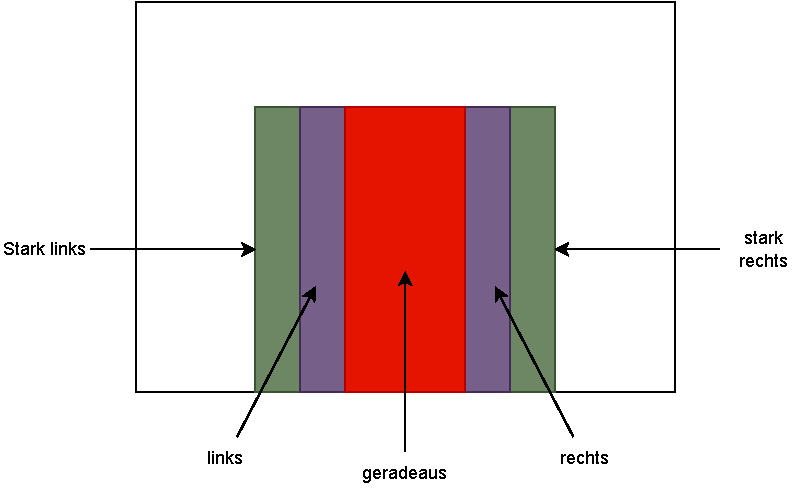
\includegraphics[width=0.7\linewidth]{concept/henseler-aufbau-kopf.pdf}
\caption{Einteilung der Bounding Box des Kopfes (grün dargestellt) in Zonen. Die blaue Zone hat eine Größe von 70\% der grünen Zonen. Die rote Zone hat eine Größe von 40\% der grünen Zone. Quelle: Abbildung nach \cite{bachelor:henseler:gaze-ebikes}.}
\label{fig:related:henseler:box}
\end{figure}

Für die Bewertung dieses Ansatzes wurden insgesamt 160 Minuten Videomaterial aufgezeichnet, das drei verschiedene Personen zeigt. Es wird darauf hingewiesen, dass in den meisten Videos die abgebildete Person eine Sonnenbrille trägt. Alle Videos wurden bei sonnigem oder leicht bewölktem Wetter aufgenommen. Andere Tageszeiten oder Wetterbedingungen wurden nicht berücksichtigt, da der von Henseler beschriebene Ansatz zur Gesichtserkennung nur bei einem gut beleuchteten Gesicht funktioniert. Bei stark bewölktem Himmel stellt die automatische Helligkeitsanpassung der Kamera des Smartphones laut Henseler ein Problem dar, da dadurch das Gesicht nicht ausreichend hell genug ist, um es zu erkennen. 

Aus den aufgezeichneten Videos wurden in regelmäßigen Abständen 1.516 Einzelbilder ausgewählt und separat gespeichert. Anschließend hat Henseler diese manuell in eine der acht oben genannten Kategorien eingeordnet, um eine Ground Truth zu erstellen. Ein Problem, das während der Erstellung der Ground Truth aufgetreten ist, war die Einordnung von Randfällen, bei denen es beispielsweise schwierig war zu entscheiden, ob die abgebildete Person nach links oder stark nach links schaut. Eine interessante Tendenz, die an den Daten der Ground Truth ersichtlich wird, ist, dass nur in jeweils zwei Fällen die Personen links oder rechts auf den Lenker geschaut haben, während insgesamt 49 Mal auf die Mitte des Lenkers (Smartphone) gesehen wurde. Dies weist darauf hin, dass Radfahrende vor allem auf ihr Smartphone schauen, wenn sie ihren Blick vom Straßenverkehr abwenden.

Nach der Erstellung der Ground Truth wurden die Bilder von dem implementierten Ansatz von Henseler verarbeitet. Dabei wurden die erkannten Gesichtsmerkmale in jedem Bild markiert und separat gespeichert. Diese Bilder wurden anschließend ebenfalls manuell ausgewertet. Dabei wurde für jedes Merkmal die binäre Entscheidung getroffen, ob das Merkmal richtig erkannt wurde oder nicht. Diese Entscheidung basierte auf der Einschätzung von Henseler.  

Das Ergebnis war, dass nur in 964 Bildern ein Gesicht erkannt werden konnte. Da die weitere Erkennung der Blickrichtung auf dem erkannten Gesicht basiert, kann somit bei den restlichen 552 Bilder keine Aussage darüber getroffen werden, wohin die dargestellte Person schaut, was eine große Schwäche des Ansatzes von Henseler ist.

Die weitere Auswertung wurde daher nur für die Bilder mit erkanntem Gesicht fortgesetzt. Von den 964 Bildern mit erkanntem Gesicht wurden bei 805 Bildern die Blickrichtung entsprechend der Ground Truth richtig klassifiziert. Die meisten Fehler sind auf eine falsche Erkennung der Nase oder des Mundes zurückzuführen. Die größten Ungenauigkeiten traten bei der Erkennung der Kategorie \textit{Lenker mitte} (Smartphone) auf. Von insgesamt 49 Bildern konnte die Kategorie nur bei 31 Bildern richtig zugeordnet werden.

Zusammenfassend kann gesagt werden, dass es Henseler gelungen ist, eine Blickrichtungserkennung von Radfahrenden zu realisieren. Mit dieser lassen sich gute Ergebnisse erzielen, wenn in einem Bild ein Gesicht erkannt werden kann. Eine besondere Stärke ist, dass teilweise verdeckte Gesichter, wie zum Beispiel durch Sonnenbrillen, erkannt werden können. Für einen Einsatz im Rahmen der PrioBike-App ist dieser Ansatz jedoch nicht geeignet. Dies liegt zum einen an der zusätzlichen Hardware in Form der Halterung des Smartphones am Fahrradrahmen und dem notwendigen gelben Klebestreifen am Fahrradhelm, ohne die der Ansatz nicht funktioniert. Eine weitere Schwäche ist, dass keine Aussage über die Blickrichtung getroffen werden kann, wenn kein Gesicht erkannt wurde, was bei Henseler bei gut einem Drittel aller Bilder der Fall ist. Außerdem ist für das PrioBike-Projekt vor allem wichtig zu erkennen, wann die Person auf das Smartphone schaut, was bei Henselers Ansatz die schlechtesten Ergebnisse lieferte. Die generelle Idee, die Blickrichtung anhand der Kopfrotation zu bestimmen, wird jedoch als vielversprechend angesehen und soll in dieser Arbeit aufgegriffen werden.

\section{Blickrichtungsbestimmung}\label{sec:related:gaze}

Im Folgenden werden Arbeiten vorgestellt, die sich mit verschiedenen Methoden zur Blickrichtungsbestimmung beschäftigen. Dabei werden sowohl Arbeiten speziell für Smartphones als auch allgemeine Methoden zur Blickrichtungsbestimmung betrachtet.

\subsection{MobiGaze}\label{sec:related:gaze:model:mobigaze}

Eine frühe Arbeit, die sich mit der Bestimmung der Blickrichtung auf Smartphone-Displays beschäftigt, ist die Arbeit von Nagamatsu et al. \cite{paper:mobigaze}. Da die einhändige Bedienung von Smartphones umständlich ist, wollten die Autoren einen Ansatz entwickeln, der die Blickrichtung einer Person nutzt, um eine Interaktion mit dem Smartphone zu ermöglichen. Zu diesem Zweck entwickelten Nagamatsu et al. \textit{MobiGaze}. Dabei handelt es sich um ein System, das aus zwei zusätzlichen Kameras und einer Infrarot-LED besteht, die am Smartphone angebracht werden. Mit diesen kann die dreidimensionale Blickrichtung des Menschen bestimmt werden. \textit{MobiGaze} ist so konzipiert, dass es dabei egal ist, wie die Person das Smartphone hält, solange die Augen von den Kameras erfasst werden können. Da die Rechenleistung von Smartphones damals noch nicht ausreichte, um die Berechnungen direkt auf dem Gerät durchzuführen, war bei diesem Ansatz zusätzlich ein Computer notwendig. Dieser hat die Berechnung der Blickrichtung durchgeführt und das Ergebnis an das Smartphone übermittelte.  

Mit dieser Interaktionsmethode stellen die Autoren einige mögliche Anwendungen vor, die darauf basieren, eine Auswahl anhand des Blicks zu treffen und diese in Kombination mit einem Druck auf das Smartphone zu bestätigen \cite{paper:mobigaze}. Damit zeigen die Autoren, dass eine dreidimensionale Blickrichtungsbestimmung für den Einsatz auf Smartphones möglich ist, auch wenn diese Methode auf zusätzlicher Hardware basiert, was sie für die Blickrichtungsbestimmung von Radfahrenden ungeeignet macht. 

\subsection{WebGazer}\label{sec:related:webgazer}\label{sec:related:gaze:appearance:webgazer}

Eine Arbeit, die sich damit beschäftigt, die Blickrichtungsbestimmung der Allgemeinheit zugänglich zu machen, ist die Arbeit von Papoutski et al. \cite{paper:webgazer}, in der sie \textit{WebGazer} vorstellen. Bei dieser Arbeit handelt es sich um eine JavaScript-Bibliothek, die in jede beliebige Webseite eingebunden werden kann. Mit \textit{WebGazer} können die Punkte auf dem Bildschirm ermittelt werden, die eine Person beim Betrachten einer Webseite ansieht. \textit{WebGazer} ist dabei nicht auf spezielle zusätzliche Hardware angewiesen, sondern ermöglicht die Blickrichtungsbestimmung mittels einer Webcam. 

Die Blickrichtungsbestimmung funktioniert dabei so, dass zunächst die Augen der Person im Bild der Webcam erkannt werden\footnote{In ihrer Arbeit verwenden Papoutsaki et al. drei verschiedene Methoden, um die Augen zu erkennen. Diese sind \textit{clmtrackr} \url{https://github.com/auduno/clmtrackr} (Abgerufen am 08.11.2023), \textit{js-objectdetect} \url{https://github.com/mtschirs/js-objectdetect} (Abgerufen am 08.11.2023), und \textit{tracking.js} \url{https://trackingjs.com/} (Abgerufen am 08.11.2023)}. Anhand der erkannten Augen kann die Blickrichtung anschließend mit zwei verschiedenen Methoden bestimmt werden. Bei dem ersten Ansatz wird die Position der Pupille des Auges erkannt, anhand derer die Bildschirmkoordinaten linear geschätzt werden. 

Für den zweiten Ansatz untersuchten Papoutski et al. den Zusammenhang zwischen den Blicken und den Interaktionen von Menschen mit einer Website. Zunächst wurden Mausklicks untersucht. Die Autoren stellten fest, dass Personen dorthin schauen, wohin sie klicken. Anschließend untersuchten sie die Mausbewegungen und stellten fest, dass diese den Blicken mit einer leichten Verzögerung folgen. Mit diesen Erkenntnissen und einem mehrdimensionalen Merkmalsvektor, den die Autoren aus dem Bild der Augen extrahierten, können so mittels einer Regressionsfunktion die Bildschirmkoordinaten bestimmt werden, auf die die Person schaut. 

Da die Implementierung von \textit{WebGazer} frei zugänglich ist und einfach in jede Webseite integriert werden kann, könnte diese Methode für die Bestimmung der Blickrichtung auf einem Smartphone implementiert werden. Damit bietet \textit{WebGazer} eine Möglichkeit, die Stellen des Displays zu identifizieren, auf die Radfahrende während der Fahrt schauen. Es ist jedoch unklar, ob mit dieser Methode unterschieden werden kann, ob eine Person auf das Display schaut oder nicht.

\subsection{Übersicht über Deep Learning Appearance-Based Methoden}\label{sec:related:gaze:appearance}

Die Bestimmung der Blickrichtung von Menschen mithilfe von Deep Learning Appearance-Based Methoden ist ein Thema, mit dem sich einige Forschungsarbeiten beschäftigen. Cheng et al. geben in ihrer Arbeit \cite{paper:basics:survey} einen Überblick über den aktuellen Stand der Forschung zu diesen Methoden.

Dafür präsentieren die Autoren zunächst die gängigen Schritten, die während der Umsetzung dieser Methode ausgeführt werden. Nach der Aufnahme eines Bildes einer Person mit einer Kamera ist es zunächst erforderlich, das Gesicht oder die Augen dieser Person innerhalb des Bildes zu erkennen. Dadurch kann das Bild auf den für die Betrachtung relevanten Bereich des Gesichts zugeschnitten werden, wodurch unwichtige Informationen aus dem Rest des Bildes eliminiert werden können.

Cheng et al. beschreiben darüber hinaus ein Verfahren, mit dem weitere Störfaktoren aus dem Bild entfernt werden können. Diese Störfaktoren entstehen vor allem dadurch, dass sich die Personen bei Appearance-Based Methoden frei bewegen können. Dadurch ist eine große Variation der Kopfdrehung möglich. Die Drehung des Kopfes um die Längsachse kann bei solchen Verfahren jedoch ignoriert werden, da sich die generelle Orientierung des Gesichts zur Kamera durch sie nicht ändert. Außerdem kann die Entfernung des Gesichts zur Kamera während der Aufnahme der Bilder variieren. Das oben genannte Verfahren von Cheng et al. vermeidet diese beiden Störfaktoren. Dazu wird zunächst ein Referenzpunkt im Gesicht der Person festgelegt. Anschließend wird die Kamera virtuell so verschoben, dass sie sich direkt über diesem Referenzpunkt befindet. Anschließend wird das Bild so gedreht, dass die Drehung des Kopfes um die Längsachse aufgehoben wird. Im letzten Schritt wird das Bild so skaliert, dass das Gesicht einen festen virtuellen Abstand zur Kamera hat \cite{paper:basics:survey}. Das Verfahren ist beispielhaft in der Abbildung \ref{fig:related:normalisierung} dargestellt.

\begin{figure}
    \centering
    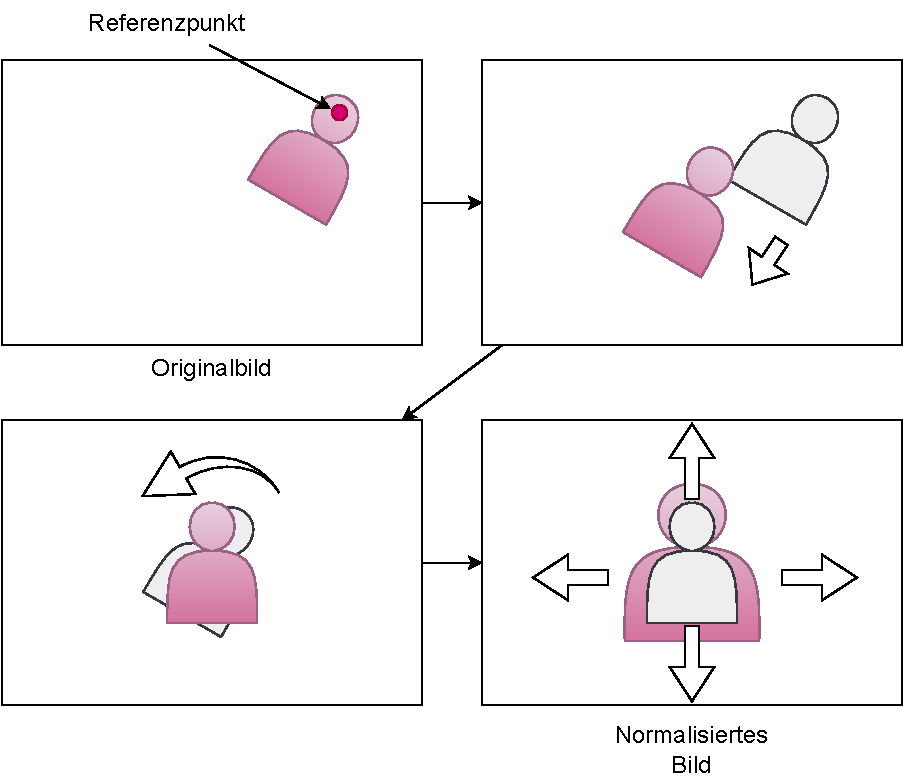
\includegraphics[width=0.8\linewidth]{related/normalisierung.pdf}
    \caption{Beispielhafte Darstellung der Normalisierung von Bildern. Quelle: Abbildung nach \cite{paper:basics:survey}}
    \label{fig:related:normalisierung}
\end{figure}

Das normalisierte Bild wird dann von einem neuronalen Netz verarbeitet, um auf die Blickrichtung der Person zu schließen. Für diese Aufgabe eignen sich besonders Convolutional Neural Networks \cite{paper:basics:survey, paper:cnn, diplom:matthes}. Eine wichtige Entscheidung, die dabei getroffen werden muss, ist die Wahl des Datensatzes, der als Grundlage für das Convolutional Neural Network verwendet wird. Cheng et al. geben in ihrer Arbeit \cite{paper:basics:survey} einen Überblick über verschiedene Datensätze. Je nach Anwendungsfall sind verschiedene Datensätze unterschiedlich gut geeignet. Eine Auswahl dieser Datensätze wird im weiteren Verlauf des Kapitels vorgestellt.

Die Vorhersage eines solchen Convolutional Neural Networks ist dann, je nach Wahl der Trainingsdaten, ein zweidimensionaler Punkt auf einem Bildschirm oder eine dreidimensionale Blickrichtung, die durch einen Pitch- und einen Yaw-Winkel angegeben wird \cite{paper:basics:survey}. Es ist zu beachten, dass sich die Vorhersage auf das normalisierte Gesicht bezieht, wenn die Bilder normalisiert wurden. Die entsprechenden Ergebnisse müssen daher umgerechnet werden, damit sie dem tatsächlich dargestellten Gesicht entsprechen.

Im Folgenden werden verschiedene Implementierungen von Convolutional Neural Networks sowie Datensätze vorgestellt, die für das Training verwendet werden können.

\subsubsection{Columbia}\label{sec:related:gaze:appearance:gaze-locking}

Smith et al. stellen in ihrer Arbeit \cite{paper:columbia} den \textit{Columbia} Datensatz vor. Dieser besteht aus 5.880 Bildern von 56 verschiedenen Personen, die unter Laborbedingungen aufgenommen wurden. Der Datensatz zeigt die Teilnehmenden in einer von fünf verschiedenen fixierten Kopfpositionen, bei denen der Kopf entlang der Vertikalachse gedreht wurde. Für jede der fünf Kopfpositionen wurden dann 21 verschiedene Ziele von den Teilnehmenden betrachtet. Somit können für jede Kopfposition 21 verschiedene Blickwinkel dargestellt werden. Durch die Fixierung des Kopfes, das Wissen, wohin die Person schaut und die Position der Kamera konnte für alle aufgenommenen Bilder ein dreidimensionaler Blickrichtungsvektor gespeichert werden, der als Ground Truth verwendet wird.

Ziel war es, mittels dieses Datensatzes einen Ansatz zu ermöglichen, den sie \textit{Gaze Locking} \cite{paper:columbia} nennen. Der Ansatz basiert auf der Tatsache, dass wir Menschen sehr gut erkennen können, ob eine Person uns ansieht oder nicht. Wir haben allerdings größere Schwierigkeiten, genau zu bestimmen, wohin eine Person schaut, wenn sie uns nicht ansieht. Daher wollten die Autoren das Problem der Blickrichtungsbestimmung vereinfachen, indem sie es zu einem binären Problem machen. Sie wollten anhand des Bildes einer Person entscheiden, ob diese Person in die Kamera schaut oder nicht.

Dafür trainierten sie anhand des Datensatzes ein Modell, das diese binäre Entscheidung treffen sollte. Das Modell erzielte sehr genaue Ergebnisse, auch bei großen Abständen zwischen Person und Kamera. Generell konnte die Arbeit zeigen, dass das Ziel der binären Entscheidung, ob eine Person in die Kamera schaut oder nicht, mithilfe des Modells umgesetzt werden konnte.
Der verwendete Datensatz von Smith et al. ist jedoch aufgrund der geringen Variation der Kopfpositionen nicht für die Bestimmung der Blickrichtung von Radfahrenden geeignet. Dies liegt vor allem daran, dass der Datensatz keine Variation der Kopfdrehung entlang der Querachse enthält. Aus Sicht der Innenkamera eines Smartphones ist jedoch vor allem die Kopfdrehung entlang der Querachse entscheidend dafür, ob Radfahrende auf das Smartphone schauen oder nicht.

\subsubsection{MPIIGaze \& MPIIFaceGaze}\label{sec:related:gaze:appearance:mpiigaze}

In einer Arbeit von Zhang et al. \cite{paper:mpiigaze, paper:mpiigaze-old} wird der \textit{MPIIGaze} Datensatz vorgestellt. Ziel der Arbeit war es, einen Datensatz zu entwickeln, der Menschen bei der Benutzung von Laptops in normalen Alltagssituationen zeigt und somit eine größere Variation von Kopfdrehungen, Hintergründen und Lichtverhältnissen darstellen kann. Dies wurde erreicht, indem 15 verschiedene Personen über einen längeren Zeitraum zu zufälligen Tageszeiten einen Punkt auf dem Bildschirm ihres Laptops fixierten. Dabei wurden Aufnahmen mit der Webcam des Laptops gemacht. Insgesamt wurden so 213.659 Bilder in verschiedenen Situationen aufgenommen. Für alle diese Bilder wurde ein dreidimensionaler Blickrichtungsvektor als Ground Truth bestimmt. 

Der Datensatz zeigt daher eine größere Variation der Kopfdrehung und der Lichtverhältnisse als der \textit{Columbia} \cite{paper:columbia} Datensatz. Aufgrund des notwendigen Blickkontakts der abgebildeten Person mit dem Bildschirm des Laptops ist der Datensatz jedoch in den abgebildeten Kopfdrehungen dennoch eingeschränkt. Der Blickwinkel einer Laptop-Webcam auf die Person vor ihr ist in den meisten Fällen nicht vergleichbar mit dem Blickwinkel eines Smartphones am Fahrradlenker auf Radfahrende. Es ist daher davon auszugehen, dass eine Verwendung des Datensatzes für den Anwendungsfall der PrioBike-App nicht geeignet ist.

Anhand ihres Datensatzes haben Zhang et al. \cite{paper:mpiigaze} anschließend ein Convolutional Neural Network entwickelt. Dazu wurden die Bilder des Datensatzes zunächst vorverarbeitet. Zuerst wurde das Gesicht innerhalb des Bildes identifiziert. Anschließend wurden verschiedene Gesichtspunkte in Form von zweidimensionalen Bildkoordinaten bestimmt \cite{paper:dlib}. Um den Einfluss der Gesichtsmerkmalserkennung auf die Ergebnisse des Convolutional Neural Networks zu untersuchen, wurden die korrekten Gesichtsmerkmale in einem Teil des Datensatzes bestimmt. Dazu wurden die Gesichtsmerkmale zunächst automatisch erkannt und anschließend von einem Menschen manuell korrigiert. Nach der Erkennung der Gesichtsmerkmale wurden diese verwendet, um die Augen der Person aus dem Bild zu extrahieren. Daraufhin wurde ein dreidimensionales Modell eines Kopfes erstellt, das auf dem Durchschnitt der im Datensatz gezeigten Personen basiert. Dieses Modell wurde verwendet, um die dreidimensionale Position der zweidimensionalen Bildkoordinaten \cite{paper:epnp} zu bestimmen. Mit diesem Verfahren konnten eine Rotationsmatrix und ein Translationsvektor bestimmt werden, die dann zur Normalisierung der Bilder mit der von Cheng et al. \cite{paper:basics:survey} vorgestellten Methode verwendet wurden. Aus dieser Normalisierung berechnen Zhang et al. einen Rotationsvektor $h$, der die Rotation des normalisierten Gesichts angibt. Da die Normalisierung die Rotation um die Längsachse eliminiert, kann der Vektor als zweidimensional betrachtet werden. Anhand der erkannten Gesichtsmerkmale werden dann die Augen aus dem Bild extrahiert. Mit $h$ und den Bildern der Augen wird dann das \cnn trainiert, um eine dreidimensionale Blickrichtung des normalisierten Kopfes zu bestimmen, die dann wieder in das ursprüngliche Koordinatensystem vor der Normalisierung umgerechnet werden kann.

In einer späteren Arbeit \cite{paper:mpiifacegaze} haben Zhang et al. untersucht, wie die Ergebnisse des Modells verbessert werden können, wenn nicht nur einzelne Augenbilder, sondern das gesamte Gesicht als Input verwendet wird. Diese Untersuchungen zeigten, dass die Verwendung des gesamten Gesichts die Qualität der Vorhersagen deutlich verbessern kann. Eine besonders wichtige Erkenntnis ihrer Arbeit war, dass das Modell vor allem bei schwierigen Lichtverhältnissen und extremen Kopfdrehungen deutlich bessere Ergebnisse erzielen konnte, was eine sehr wichtige Erkenntnis für die Anwendung einer solchen Methode im Rahmen der PrioBike-App ist.

\subsubsection{GazeCapture}\label{sec:related:gaze:appearance:gazecapture}

Krafka et al. stellen in ihrer Arbeit den Datensatz \textit{GazeCapture} vor \cite{paper:gazecapture}. Dieser Datensatz umfasst Bilder von 1.474 verschiedenen Personen und ist somit der Datensatz mit der größten Anzahl von verschiedenen Teilnehmenden. Er besteht aus 2.400.000 Bildern von Personen im täglichen Leben. Aufgenommen wurden die Bilder mit den Smartphones und Tablets der Personen. Der Datensatz spiegelt damit eine sehr große Diversität von verschiedenen Gesichtern, Accessoirs, Hintergründen und Beleuchtungebedingungen wieder. Dafür wurde eine Anwendung entwickelt, welche die Personen auf ihrem Gerät installieren konnten. Diese Anwendung zeigte den Teilnehmenden einen Punkt auf dem Bildschirm ihres Geräts, den sie fixieren sollten. Zusätzlich wurden die Teilnehmenden durch die Anwendung dazu motiviert, ihren Kopf zu bewegen und den Abstand zwischen dem Gerät und dem Kopf zu vergrößern. Für alle der dabei entstanden Bilder wurde die entsprechende Koordinate des Punktes auf dem Bildschirm, die Orientierung des Geräts sowie die Art des Geräts als Ground Truth gespeichert.

Aufbauend auf \textit{GazeCapture} entwickelten Krafka et al. \textit{iTracker} \cite{paper:gazecapture}. Dabei handelt es sich um einen \cnn, das aus den Bildern des Gesichts und der Augen einer Person und einer binären Maske, die die relative Position des Kopfes im Originalbild wiedergibt, eine zweidimensionale Koordinate für ein Gerät ermitteln kann. Dazu haben sie verschiedene Experimente durchgeführt und unter anderem \textit{iTracker*} entwickelt. Dieses Modell verwendet das Daten über die Orientierung und die Art des verwendeten Geräts, um die Ergebnisse zu maximieren. Mit ihrem Ansatz erzielten Krafka et al. einen durchschnittlichen Fehler von 1,04 cm bei Smartphones und 1,69 cm bei Tablets \cite{paper:gazecapture}.

Dieser Datensatz und das damit trainierte Modell beinhalten jedoch aufgrund der Art der Datenerhebung mit dem durchgehenden Blickkontakt der Person mit dem Display nur eine eingeschränkte Variation der Kopfdrehung, die nicht mit der Kopfdrehung von Radfahrenden vergleichbar ist, was diesen Datensatz für eine Verwendung in dieser Arbeit ungeeignet macht.

\subsubsection{TabletGaze}\label{sec:related:gaze:appearance:tabletgaze}

Ein weiterer Datensatz, der speziell mit Tablets aufgenommen wurde, wird von Huang et al. in ihrer Arbeit \cite{paper:tabletgaze} vorgestellt. Dabei handelt es sich um den \textit{Rice TabletGaze} Datensatz. Ziel des Datensatzes war es, eine unkalibrierte Bestimmung der Blickrichtung von Personen auf einem Tablet zu ermöglichen. Dazu wurde ein Datensatz erstellt, der auf 51 verschiedenen Personen basiert. Von diesen Personen wurden Videos mit der Innenkamera des Tablets aufgenommen, während sie das Tablet benutzten. Während der Aufnahme konnten sich die Teilnehmenden frei bewegen, es wurde lediglich eine von vier allgemeinen Körperhaltungen vorgegeben. Diese Körperhaltungen waren Sitzen, Liegen, Stehen und eine entspannte Haltung auf einem Sofa. Während der Nutzung des Tablets sollten die Probanden einen zufällig auf dem Bildschirm platzierten Punkt verfolgen. Mithilfe dieses Punktes wurde für jedes aufgenommene Bild die zweidimensionale Koordinate des Punktes als Ground Truth gespeichert.

Anschließend wurden die aufgenommenen Bilder gefiltert. So wurden Aufnahmen entfernt, die kurz nach dem Positionswechsel des Punktes gemacht wurden, um die Übergangsphase, in der sich die Person auf den neuen Punkt fixiert, zu eliminieren. Außerdem wurde versucht, die Augen der Person im Bild zu erkennen, um diese zu dem Datensatz hinzufügen zu können. Können keine Augen erkannt werden, werden auch diese Bilder aussortiert. Anschließend wird anhand der durchschnittlichen Pixelintensität im Bereich der Augen erkannt, ob die Augen geschlossen sind oder nicht. Wenn ein geschlossenes Auge erkannt wurde, wurde das entsprechende Bild sowie die Bilder direkt davor und danach entfernt. Auf diese Weise entstand ein Datensatz mit insgesamt 100.000 Einträgen.

In diesem Datensatz ist zwar auch eine Variation der Kopfdrehung enthalten, diese wird jedoch durch den ständigen Blickkontakt der Person mit dem Display des verwendeten Gerätes eingeschränkt, was diesen Datensatz für die Verwendung der Blickrichtungsbestimmung von Radfahrenden für diese Arbeit ungeeignet macht.

\subsubsection{RT-GENE}\label{sec:related:gaze:appearance:rt-gene}

Fischer et al. präsentieren in ihrer Arbeit den \textit{RT-GENE} Datensatz \cite{paper:rt_gene}. Dieser wurde dadurch motiviert, dass existierende Datensätze keine große Varianz bezüglich der Entfernung der Personen zur Kamera aufweisen. Der Datensatz besteht aus 15 verschiedenen Personen, von denen 122.531 Bilder aufgenommen wurden. Der Datensatz wurde unter Laborbedingungen aufgenommen. Dazu wurde eine Person in einem Raum platziert. Dieser Person wurde eine Halterung auf den Kopf gesetzt, in die ein Eye-Tracker integriert wurde. Die Aufgabe dieser Halterung ist es, die Blickrichtung zu messen. So kann der Kopf frei bewegt werden, ohne ein bestimmtes Ziel anvisieren zu müssen. Dieser Rahmen wurde so groß gestaltet, dass möglichst wenig von den Augen verdeckt wird. An dieser Halterung wurden vier Marker befestigt. Anhand dieser Marker konnte ein Motion-Capture-System die Kopfdrehung der Versuchspersonen ermitteln. Mit diesem Aufbau war es möglich, Bilder der Testperson aufzunehmen, bei denen die Testperson weiter von der Kamera entfernt stand und den Kopf frei bewegen konnte. Aus der gemessenen Blickrichtung des Eye-Trackers und der gemessenen Kopfhaltung des Motion-Capture-Systems konnte so für jedes Bild ein dreidimensionaler Blickrichtungsvektor ermittelt und gespeichert werden.

In diesen Bildern der Personen ist jedoch das Gestell mit dem integrierten Eye-Tracker zu erkennen, was in einem alltäglichen Anwendungsfall natürlich nicht der Fall wäre. Daher wird das Gestell mittels eines Generative Adversial Network (GAN) \cite{paper:gan} aus dem Originalbild entfernt. Der Datensatz wurde weiter gefiltert, indem Bilder entfernt wurden, bei denen die Kopfdrehung zu groß war, um beide Augen der Person zu erkennen. Bilder mit geschlossenen Augen wurden ebenfalls entfernt.

Der Datensatz zeigt ein breiteres Spektrum an Kopfdrehungen als die vorherigen Datensätze. Allerdings wurden die Bilder unter Laborbedingungen bei gleicher Beleuchtung aufgenommen, was für den Anwendungsfall der Blickrichtungsbestimmung beim Radfahren nicht ideal ist. 

Weiter stellen Fischer et al. einen Ansatz vor, diesen Datensatz zur Bestimmung der Blickrichtung von Personen zu verwenden \cite{paper:rt_gene}. Dazu werden zunächst markante Gesichtsmerkmale im Bild erkannt \cite{paper:mtcnn}. Anhand der erkannten Gesichtspunkte werden die Augen aus dem Originalbild ausgeschnitten. Anschließend wird das von Cheng et al. vorgestellte Verfahren zur Normalisierung der Bilder der Augen \cite{paper:basics:survey} angewendet. Diese werden separat in einen VGG-16 \cnn geladen. Damit ist es möglich, die dreidimensionale Blickrichtung einer Person durch den Pitch- und Yaw-Winkel zu bestimmen. Die Methode lieferte sehr gute Ergebnisse und konnte auch die maximale Performance anderer Datensätze, wie zum Beispiel \textit{MPIIGaze}, verbessern.

\subsubsection{Gaze360}\label{sec:related:gaze:appearance:gaze360}

Kellnhofer et al. stellen in ihrer Arbeit \cite{paper:gaze360} den Datensatz \textit{Gaze360} vor. Dabei handelt es sich um einen Datensatz, der sowohl Außen- als auch Innenaufnahmen enthält und eine große Variation von Kopfdrehungen zeigt. Der Datensatz besteht aus 238 verschiedenen Personen mit insgesamt 172.000 Aufnahmen. Zur Aufnahme der Bilder wurde eine 360°-Kamera verwendet. Um diese Kamera herum wurden verschiedene Personen in einem Abstand von zwei bis drei Metern aufgestellt. Eine weitere Person trägt ein Schild. Auf diesem Schild ist zum einen ein Code \cite{paper:april-tag} und zum anderen ein großer Punkt zu sehen. Auf diesen Punkt sollen die Teilnehmenden schauen, während die Person mit dem Schild um sie herumgeht. Der Aufnahmeprozess wurde dabei in zwei verschiedene Phasen unterteilt. In der ersten Phase war es den Teilnehmenden erlaubt, ihren Kopf zu bewegen, um so eine große Reichweite von verschiedenen Kopfdrehungen im Datensatz zu ermöglichen. In der zweiten Phase durften die Teilnehmenden ihren Kopf nicht bewegen und sollten den Punkt nur mittels der Augen verfolgen, um so auch eine große Reichweite von Blickwinkeln zu ermöglichen. Das Schild mit dem Punkt war dabei immer so ausgerichtet, dass der dargestellte Code auf dem Schild zur Kamera zeigt. Anhand des Codes wurde das Schild später in den Aufnahmen erkannt. So konnten Rückschlüsse auf die dreidimensionale Position des Punkt geschlossen werden. So konnte für jede Aufnahme ein dreidimensionaler Blickrichtungsvektor bestimmt werden. 
Durch die große Variation der Kopfdrehungen und dem Vorhandensein von Außenaufnahmen könnte dieser Datensatz gut geeignet sein, um eine Blickrichtungsbestimmung von Radfahrenden zu ermöglichen.

Darüber hinaus stellen Kellnhofer et al. in ihrer Arbeit  \cite{paper:gaze360} ein Modell zur Blickrichtungsbestimmung vor. Dieses basiert auf der Tatsache, dass die Bestimmung der Blickrichtung ein kontinuierlicher Prozess ist und daher die Blickrichtungen aufeinanderfolgender Bilder voneinander abhängig sind. Dafür verwenden wird die Autoren ein \cnn, bei dem als Eingabe sieben aufeinanderfolgende Bilder mit Gesichtern einer Person verwendet werden. Diese werden dann in bidirektionale Long Short-Term Memory Capsules (LSTM) \cite{paper:lstm} gegeben. Mittels einer Fully Connceted-Schicht wird dann die Blickrichtung vorhergesagt. Das Modell kann somit für die Vorhersage des aktuellen Bildes auch die Vorhersagen der drei vorhergehenden und der drei nachfolgenden Bilder zur Blickrichtungsbestimmung verwenden.

\subsubsection{L2CS-net}\label{sec:related:gaze:appearance:l2cs}

Abdelrahman et al. stellen in ihrer Arbeit \cite{paper:l2csnet} ein robustes \cnn zur Bestimmung der Blickrichtung in freien Umgebungen vor. Dazu verwenden sie die Datensätze \textit{MPIIGaze} und \textit{Gaze360}. Die Bilder der Datensätze werden zunächst mit dem von Cheng et al. \cite{paper:basics:survey} präsentierten Verfahren zur Normalisierung der Bilder verarbeitet. Für die Blickrichtungsbestimmung, verwenden die Autoren ein ResNet-50 \cnn. Das besondere an ihrem Ansatz ist, dass der Pitch- und der Yaw-Winkel, die die dreidimensionale Blickrichtung angeben, jeweils separat von einem Fully Connected Layer vorhergesagt werden. Mit diesem Ansatz konnten sie im Vergleich zu anderen Arbeiten in beiden Datensätzen den geringsten Blickrichtungsfehler erzielen. Ihre Implementierung des Verfahrens ist öffentlich zugänglich\footnote{\url{https://github.com/Ahmednull/L2CS-Net} (Abgerufen am 09.11.2023)}.


\subsubsection{ETH-XGaze}\label{sec:related:eth-xgaze}\label{sec:related:gaze:appearance:eth-xgaze}

In der Arbeit von Zhang et al. \cite{paper:eth-xgaze} wird der Datensatz \textit{ETH-XGaze} vorgestellt. Ziel der Arbeit war es, einen robusten Datensatz für die Bestimmung der Blickrichtung bei einer großen Variation von Kopfposen zu erstellen, da vorherige Arbeiten wie zum Beispiel \textit{MPIIGaze} \cite{paper:mpiigaze} oder \textit{RT-Gene} \cite{paper:rt_gene} sehr limitiert sind, was die Reichweite der Kopfrotation betrifft.

Der Datensatz von Zhang et al. umfasst 1.083.492 Bilder mit den dazugehörigen dreidimensionalen Blickrichtungen von insgesamt 110 Teilnehmenden im Alter von 19 bis 41 Jahren. Die Teilnehmenden stammen aus diversen Ethnien. 47 der Teilnehmenden sind weiblich, 63 sind männlich. Für die Erstellung des Datensatzes wurden die Teilnehmenden in einem Abstand von etwa einem Meter vor einen Bildschirm mit einer Größe von 120 $\times$ 100 cm platziert. Dabei wurden die Teilnehmenden von insgesamt vier Lichtquellen beleuchtet, welche links und rechts neben dem Bildschirm platziert wurden. Mit diesen Lichtquellen lassen sich durch das Ein- und Ausschalten einzelner Lichtquellen 16 verschiedene Beleuchtungsbedingungen simulieren. Um die Kopfrotation der Teilnehmenden während der Aufnahme zu messen, wurde der Kopf der Probanden fixiert. Die Teilnehmenden wurden dazu angehalten, ihren Kopf während des Experiments nicht zu bewegen. Um dennoch eine große Variation von Kopfposen zu ermöglichen, wurden die Teilnehmenden von 18 verschiedenen Kameras aufgenommen, welche alle einen anderen Blickwinkel auf die Probanden zeigen. Diese Kameras nehmen Bilder mit einer Auflösung von 6000 $\times$ 4000 Pixeln auf. 

Der Datensatz von Zhang et al. enthält im Vergleich zu den bisherigen Datensätzen die größte Vielfalt an Kopfrotationen und Blickwinkeln. Außerdem variieren die Einträge des Datensatzes stark in der Beleuchtung. Aufgrund der zu erwartenden Vielfalt an Kopfrotationen der Radfahrenden sowie der vielen unterschiedlichen Lichtbedingungen während der Fahrt ist dieser Datensatz vielversprechend für den Einsatz innerhalb der PrioBike-App.

Anhand des Datensatzes haben Zhang et al. anschließend ein \cnn mit einer Standard ResNet-50 Architektur trainiert. Für das Trainieren des Modells werden die Bilder vorab bearbeitet. Die Autoren beschreiben, dass dafür zunächst das Gesicht und anschließend die Gesichtsmerkmale innerhalb des Bildes erkannt werden. Um die dreidimensionale Kopfrotation der Person zu bestimmen, werden die erkannten zweidimensionalen Gesichtspunkte auf ein dreidimensionales Gesichtsmodell übertragen \cite{paper:eth-xgaze-3d-pose}. Mithilfe der dabei bestimmten Kopfrotation werden die Bilder anschließend mit der von Cheng et al. beschriebenen Methode \cite{paper:basics:survey} normalisiert.

Die Leistung des trainierten Modells wurden mit Modellen basierend auf Datensätze von anderen Arbeiten verglichen. Die Ergebnisse haben gezeigt, dass Zhang et al. mit ihrem Ansatz den geringsten Blickrichtungsfehler sowohl bei niedrigen als auch hohen Kopf- und Blickwinkeln erzielen konnten, was ebenfalls vielversprechend für den Einsatz der Arbeit im Rahmen des PrioBike-Projekts ist. 

\subsubsection{Zusammenfassung}


Cheng et al. stellen in ihrer Arbeit die allgemeine Vorgehensweise zur Bestimmung der Blickrichtung mit Deep Learning Appearance-Based Methoden vor. Darüber hinaus geben sie einen Überblick über verschiedene Implementierungen und Datensätze, die dafür verwendet werden können. Eine Übersicht über diese Datensätze ist in Tabelle \ref{tab:related:overview:gaze:angles} und Tabelle \ref{tab:related:overview:gaze:content} \cite{paper:eth-xgaze, paper:gaze360} dargestellt.

\begin{table}
\begin{tabular}{l c c c }
\toprule
                                        & \makecell{\textbf{Anzahl}\\\textbf{Personen}} & \makecell{\textbf{Variation}\\\textbf{Kopfdrehung}} & \makecell{\textbf{Variation}\\\textbf{Blickwinkel}} \\
\midrule
Columbia \cite{paper:columbia}          & 56    & 0\degree, $\pm$30\degree    & $\pm$15\degree, $\pm$10\degree  \\
MPIIGaze \cite{paper:mpiigaze}          & 15    & $\pm$15\degree, 30\degree   & $\pm$20\degree, $\pm$20\degree  \\ 
GazeCapture \cite{paper:gazecapture}    & 1.474 & $\pm$30\degree, 40\degree     & $\pm$20\degree, $\pm$20\degree  \\
RT-GENE \cite{paper:rt_gene}            & 15    & $\pm$40\degree, $\pm$40\degree  & $\pm$40\degree, -40\degree    \\
Gaze360 \cite{paper:gaze360}            & 238   & $\pm$90\degree, unknown       & $\pm$140\degree, -50\degree   \\
ETH-XGaze \cite{paper:eth-xgaze}        & 110   & $\pm$80\degree, $\pm$80\degree  & $\pm$120\degree, $\pm$70\degree \\
\bottomrule
\end{tabular}
\caption{Überblick über die vorgestellten Datensätze. Die Tabelle beinhaltet die Anzahl der Personen in einem Datensatz sowie die dargestellte maximale Kopfdrehung (Yaw, Pitch) und den maximalen Blickwinkel (Yaw, Pitch). Die angebenen Reichweiten der Kopfdrehung und Blickwinkel entstammen der Arbeit von Zhang et al. \cite{paper:eth-xgaze}. Der \textit{TabletGaze} Datensatz wird in der Arbeit von Zhang et al. \cite{paper:eth-xgaze} nicht aufgeführt.}
\label{tab:related:overview:gaze:angles}
\end{table}

\begin{table}
\begin{tabular}{l c c c c c}
\toprule
                                        & \textbf{\#Daten} & \textbf{Auflösung} & \textbf{Outdoor} & \textbf{Gaze} & \textbf{Image}  \\
\midrule

Columbia \cite{paper:columbia}          &  5.880     & $5.184 \times 3.456$ & \xmark & \textcolor{blue}{3D} & Gesicht\\
MPIIGaze \cite{paper:mpiigaze}          &  213.659   & $1.280 \times 720$   & \xmark & \textcolor{blue}{3D} & Gesicht\\ 
GazeCapture\footnote{In der Tabelle von Kellnhofer et al. \cite{paper:gaze360} als \textit{iTracker} bezeichnet.} \cite{paper:gazecapture}    &  2.445.504 & $640 \times 480$     & Teilweise & \textcolor{red}{2D} & Gesicht\\
TabletGaze\footnote{Zhang et al. nennen in ihrer Arbeit \cite{paper:eth-xgaze} keine Daten über den \textit{TabletGaze} Datensatz. Die dadurch fehlenden Daten wurden aus der Arbeit von Huang et al. \cite{paper:tabletgaze} entnommen.} \cite{paper:tabletgaze}      
                                    &  100.000   & $1.280 \times 720$   & \xmark & \textcolor{red}{2D}  & Augen \\
RT-GENE \cite{paper:rt_gene}            & 122.531    & $1.920 \times 1.080$ & \xmark & \textcolor{blue}{3D} & Gesicht\\
Gaze360 \cite{paper:gaze360}            & 172.000    & $3.382 \times 4.096$\footnote{Die hier verwendete Auflösung stammt nicht aus der Arbeit von Zhang et al. \cite{paper:eth-xgaze}, sondern aus der Arbeit von Kellnhofer et al. \cite{paper:gaze360}.} & \cmark & \textcolor{blue}{3D} & Gesicht \\
ETH-XGaze\footnote{Dieser Datensatz wurde in der Arbeit von Kellnhofer et al. nicht aufgeführt \cite{paper:gaze360}. Die Daten dieser Zeile entstammen der Arbeit von Zhang et al. \cite{paper:eth-xgaze}} \cite{paper:eth-xgaze}    & 1.083.492  & $6.000 \times 4.000$ & \xmark& \textcolor{blue}{3D} & Gesicht \\
\bottomrule
\end{tabular}
\caption{Übersicht über den Inhalt der Datensätze. Die Tabelle enthält die Größe des Datensatzes sowie die Auflösung der aufgezeichneten Daten. Die Daten in den beiden Spalten sind der Arbeit von Zhang et al. \cite{paper:eth-xgaze} entnommen. Darüber hinaus gibt die Tabelle an, ob ein Datensatz Außenaufnahmen enthält, welche Art von Ground Truth-Daten die Blickrichtung des Datensatzes angibt (2D für Bildschirmkoordinaten, 3D für Blickrichtungsvektor) und ob Bilder des gesamten Gesichts oder Bilder der Augen Teil des Datensatzes sind. Die Daten dieser drei Spalten stammen aus der Arbeit von Kellnhofer et al. \cite{paper:gaze360}}
\label{tab:related:overview:gaze:content}
\end{table}



\section{Gesichtserkennung und Gesichtsmerkmalsbestimmung}\label{sec:related:face}

Eine wichtige Teilaufgabe bei der Bestimmung der Blickrichtung ist das Erkennen des Gesichts einer Person in einem Bild und zusätzlich das Erkennen von Gesichtsmerkmalen der Person anhand des erkannten Gesichts. Diese Aufgabe findet auch Anwendung in anderen Forschungsbereichen, wie zum Beispiel der Emotionserkennung von Menschen, der Messung der Aufmerksamkeit von Autofahrenden und vielem mehr \cite{paper:face:survey}. Aus diesem Grund gibt es einige Forschungsarbeiten zu diesem Thema. 

\subsection{Übersicht über Methoden zur Erkennung von Gesichtsmerkmalen}\label{sec:related:face:survey}
In ihrer Arbeit \cite{paper:face:survey} geben Khabarlak et al. einen Überblick über den Stand der Forschung zur Erkennung von Gesichtsmerkmalen, welcher im Folgenden zusammengefasst wird.

Zunächst stellen die Autoren die wichtigsten Datensätze vor, die für das Training und die Evaluierung von Algorithmen zur Erkennung von Gesichtsmerkmalen verwendet werden. Diese Datensätze bilden jeweils eine große Variation von Gesichtsausdrücken, Lichtverhältnissen und Posen ab. Auch Bilder mit teilweise verdeckten Gesichtern sind in den Datensätzen enthalten. 

Als erstes gibt es den Datensatz \textit{300 Faces in-the-Wild (300W)} \cite{paper:300w}, der von Sagonas et al. eingeführt wurde. Er besteht aus 4.437 Bildern, die sowohl Innen- als auch Außenaufnahmen enthalten. Diese Bilder wurden halbautomatisch mit dem von Sagonas et al. in ihrer Arbeit \cite{paper:300w:ground:truth} vorgestellten Ansatz mit 68 Gesichtsmerkmalen annotiert und anschließend manuell korrigiert. Anschließend wird der \textit{Annotated Facial Landmarks in-the-Wild (AFLW)}-Datensatz von Köstinger et al. \cite{paper:aflw} vorgestellt.  Dieser Datensatz besteht aus 24.386 Bildern, die mit 21 Gesichtsmerkmalen pro Bild annotiert wurden. Ein weiterer Datensatz, \textit{Caltech Occlued Faces in the Wild (COFW)}, wird von Burgos-Artizzu et al. \cite{paper:cofw} eingeführt. Dieser besteht aus 1.852 Bildern, in denen hauptsächlich das Gesicht der abgebildeten Person durch Gegenstände oder Körperteile verdeckt ist. Die Bilder wurden mit 29 Gesichtsmerkmalen annotiert. Abschließend nennen Khabarlak et al. den \textit{Wider Facial Landmarks in-the-Wild (WFLW)} Datensatz. Dieser wurde von Wu et al. in ihrer Arbeit \cite{paper:wflw} vorgestellt. Er enthält 10.000 Bilder, welche mit 98 Gesichtsmerkmalen annotiert wurden.

Zusätzlich zu diesen vorgestellten Datensätzen gibt es Abwandlungen dieser Datensätze, in denen die genutzten Bilder zum Beispiel mit einer anderen Anzahl von Gesichtsmerkmalen annotiert wurden.

Anschließend geben Khabarlak et al. einen Überblick über die entwickelten Algorithmen zur Bestimmung von Gesichtsmerkmalen. Diese sind in Kategorien eingeteilt. Zum einen gibt es \textit{direkte} Algorithmen, deren Ergebnis eine Liste von zweidimensionalen Bildkoordinaten der einzelnen Gesichtspunkte ist. Dann gibt es den \textit{Shape-Model} Ansatz, bei dem ein dreidimensionales Modell eines Kopfes so verformt wird, dass es dem abgebildeten Kopf entspricht. Aus diesem Modell können dann beliebig viele Gesichtsmerkmale extrahiert werden. Schließlich gibt es noch den \textit{Heatmap} Ansatz. Bei diesem Ansatz wird eine Heatmap für das Bild berechnet. Die Werte der Heatmap können als Wahrscheinlichkeit für die Position eines Gesichtspunktes verwendet werden \cite{paper:face:survey}. 

Im Folgenden werden einige von Khabarlak et al. präsentierten Algorithmen zusammengefasst, die für den Anwendungsfall der PrioBike-App relevant sind. Bei dem ersten Algorithmus, handelt es sich um \textit{Ensemble of Regression Trees (ERT)}. Dieser Algorithmus gehört zu den \textit{direkten} Algorithmen. Er wird unter anderem in der Open-Source-Bibliothek \textit{dlib} \cite{paper:dlib:main, paper:dlib} verwendet, um Gesichtsmerkmale zu bestimmen. Für die Verwendung dieses Algorithmus muss zunächst eine Bounding Box des im Bild dargestellten Gesichts ermittelt werden. Bei \textit{dlib} geschieht das durch einen Ansatz, der in der Arbeit von Viola et al. \cite{paper:dlib:face} vorgestellt wird. Nach dem Erkennen des Gesichts wird als Ausgangspunkt das Modell eines Gesichts verwendet, das auf Durchschnittswerten basiert und aus 68 Gesichtspunkten besteht. Anschließend wird dieses Modell iterativ an das im Bild dargestellte Gesicht angepasst. Der Algorithmus wurde auf dem \textit{300W} Datensatz trainiert. Der Algorithmus ist einer der ersten Algorithmen, die für die Gesichtsmerkmalsbestimmung verwendet wurden. Er zeichnet sich aber durch eine hervorragende Geschwindigkeit aus, weswegen er immer noch in der aktuellen Forschung verwendet wird \cite{paper:face:survey}. Es existieren auch Implementierung dieses Algorithmus für den Einsatz auf Smartphones \cite{paper:face:survey}, wodurch er im Rahmen der PrioBike-App verwendet werden könnte. 

Ein weiterer Algorithmus ist \textit{Dense Face Alignment (DeFA)}, welcher in der Arbeit von Lui et al. \cite{paper:defa} entwickelt wurde. Die Autoren wollten mit dieser Arbeit einen Ansatz entwickeln, mit dem Gesichtsmerkmale bei extremen Kopfrotationen robust bestimmt werden können. Der dafür entwickelte Algorithmus verwendet einen \textit{Shape-Model} Ansatz. Dabei wird ein \cnn verwendet, um ein dreidimensionales Modell eines Gesichts so zu verformen, dass es dem Gesicht der dargestellten Person entspricht. Anschließend werden aus diesem Modell die Gesichtsmerkmale extrahiert. Der Algorithmus könnte im Rahmen dieser Arbeit genutzt werden, um Gesichter der Radfahrenden bei extremen Kopfrotationen zu identifizieren.

In der Arbeit von Dong et al. \cite{paper:san} wird der Ansatz \textit{Style Aggregated Network (SAN)} vorgestellt. Dabei handelt es sich um einen \textit{Heatmap}-Ansatz, der auf einem Resnet-152 Modell basiert. Dieser eignet sich laut Khabarlak et al. \cite{paper:face:survey} hervorragend zur Identifizierung von Gesichtsmerkmalen unter extremen Lichtbedingungen. Dadurch könnte der Ansatz im Rahmen dieser Arbeit genutzt werden, um die Auswirkungen von extremen Lichtbedingungen aufgrund von Wetter- und Umweltbedingungen während der Fahrt zu kompensieren.

Khabarlak et al. nennen zwei Methoden speziell für die Anwendung auf Smartphones. Die erste Methode ist \textit{Multi-task Cascaded Convolutional Neural Networks (MTCNN)}, entwickelt von Zhang et al. \cite{paper:mtcnn}. Diese Methode ermöglicht eine effiziente Bestimmung des Gesichts zusammen mit fünf Gesichtsmerkmalen. Erkannt werden dabei die Positionen des linken und rechten Auges, der Nasenspitze sowie der linke und rechte Mundwinkel. Die zweite Methode \textit{BlazeFace} wurde von Bazarevsky et al. \cite{paper:mediapipe:blazeface} entwickelt. Sie zeichnet sich vor allem durch ihre außerordentliche Geschwindigkeit aus. Auch mit diesem Ansatz können das Gesicht sowie sechs Merkmale im Gesicht wie Ohren, Augen, Nasenspitze sowie die Mitte des Mundes erfasst werden.

Durch die Untersuchungen von Khabarlak et al. konnte ein umfassender Überblick über verschiedene Gesichtserkennungsalgorithmen gewonnen werden. Dabei wurden spezielle Algorithmen herausgefiltert, die als Grundlage für die Blickrichtungsbestimmung in dieser Arbeit eingesetzt werden können.


\subsection{MediaPipe}\label{sec:related:mediapipe}\label{sec:related:face:mediapipe}

Lugaresi et al. stellen in ihrer Arbeit \cite{paper:mediapipe} \mediapipe vor. Dabei handelt es sich um ein Framework, mit dem Pipelines für Computer Vision Aufgaben erstellt werden können. \mediapipe wurde speziell für den Einsatz auf Smartphones entwickelt. Teil dieses Frameworks ist unter anderem eine vorgefertigte Pipeline zur Erkennung von Gesichtern innerhalb eines Bildes. Dabei handelt es sich um eine Kombination aus Gesichtserkennung, Bestimmung von Gesichtsmerkmalen und Verfeinerung dieser Gesichtsmerkmale.

Der erste Schritt dieser Pipeline, die Gesichtserkennung, erfolgt durch \textit{BlazeFace} \cite{paper:mediapipe:blazeface}, das bereits in Kapitel \ref{sec:related:face:survey} vorgestellt wurde. Basierend auf den Ergebnissen dieser Gesichtserkennung wird mittels eines Modells, welches von Kartynnik et al. in ihrer Arbeit \cite{paper:mediapipe:landmarks} eingeführt wurde, eine Liste dreidimensionaler Gesichtspunkte berechnet.  In einem optionalen weiteren Schritt können durch \textit{Attention Mesh}, welches von Grishchenko et al. in der Arbeit \cite{paper:mediapipe:attention} vorgestellt wurde, die Gesichtsmerkmale an markanten Stellen wie dem Mund und der Nase weiter verfeinert werden. 
Dies ermöglicht eine robuste und schnelle Erkennung von Gesichtsmerkmalen auf Smartphones mit \mediapipe und macht sie somit zu einem vielversprechenden Anwendungsgebiet für die PrioBike-App.

\section{Zusammenfassung}

In diesem Kapitel wurden relevante Arbeiten zur Blickrichtungsbestimmung von Radfahrenden vorgestellt. Zunächst wurde die Arbeit von Henseler \cite{bachelor:henseler:gaze-ebikes} diskutiert, die sich bereits speziell mit der Blickrichtungsbestimmung von Radfahrenden beschäftigt. Der von Henseler vorgestellte Ansatz, die Kopfdrehung der Radfahrenden zur Bestimmung der Blickrichtung zu nutzen, wurde als vielversprechender Ansatz für diese Arbeit identifiziert. Es wurden jedoch einige Limitationen bei der Umsetzung des Konzepts von Henseler festgestellt. So erfordert die Implementierung eine spezielle Halterung für das Smartphone. Außerdem ist die Implementierung nicht robust gegenüber wechselnden Lichtverhältnissen und funktioniert daher nur bei gutem Wetter. Zudem konnte während der Evaluation bei gut einem Drittel der Bilder mit der Implementierung keine Aussage über die Blickrichtung getroffen werden. Das entscheidende Problem der Implementierung ist jedoch, dass die größte Ungenauigkeit bei der Erkennung von Blicken auf das Smartphone besteht.

Außerdem wurden einige Arbeiten vorgestellt, die sich mit der Bestimmung der Blickrichtung von Personen beschäftigen. Insbesondere wurden Deep Learning Appearance-Based Methoden untersucht. Mit diesen Methoden kann aus einem Kamerabild die Blickrichtung einer abgebildeten Person bestimmt werden. Aus der Arbeit von Cheng et al. \cite{paper:basics:survey} konnte ein Überblick über die allgemeine Bildverarbeitung sowie einige Datensätze, die für diese Methoden verwendet werden können, gewonnen werden. Diese vorgestellten Datensätze beschäftigen sich zum einen mit der Blickrichtungsbestimmung auf Smartphones oder Laptops, wie \textit{TabletGaze} \cite{paper:tabletgaze}, \textit{GazeCaptuure} \cite{paper:gazecapture} oder \textit{MPIIGaze}. Diese sind besonders gut geeignet, um einen Blickpunkt auf einem Display zu identifizieren. Zum anderen gibt es Datensätze, die darauf ausgelegt sind, die Blickrichtung von Personen in uneingeschränkten Umgebungen zu bestimmen. Beispiele hierfür sind \textit{RT-GENE} \cite{paper:rt_gene}, \textit{Gaze360} \cite{paper:gaze360} oder \ethg \cite{paper:eth-xgaze}.

Aus der Arbeit von Zhang et al. \cite{paper:mpiifacegaze} konnte abgeleitet werden, dass für den Anwendungsfall der PrioBike-App vor allem Datensätze verwendet werden sollten, die das Gesicht der Person zeigen, da diese bei großen Kopfdrehungen und schlechten Lichtverhältnissen bessere Ergebnisse liefern als Ansätze, die nur mit den Augen des Menschen trainiert wurden.

Darüber hinaus wurden Methoden zur Erkennung von Gesichtsmerkmalen identifiziert, die für die Bestimmung der Blickrichtung wichtig sind. Dadurch konnte ein Überblick über die vorhandenen Technologien gewonnen werden. 



